% !TeX root = main.tex
%%%%%%%%%%%%%%%%%%%%%%%%% PREAMBLE %%%%%%%%%%%%%%%%%%%%%%%%%%%%%%%%
%%%%%%%%%%%%%%%%%%%%%%%% BASIC DOCUMENT SETUP %%%%%%%%%%%%%%%%%%%%%
\documentclass[a4paper]{report}
\usepackage[utf8]{inputenc}
\usepackage[english]{babel}

%%%%%%%%%%%%%%%%%%%%%%%%%% PACKAGES %%%%%%%%%%%%%%%%%%%%%%%%%%%%%%%
\usepackage{datetime}
\usepackage{datenumber}
\usepackage{parskip}
\usepackage{forest}
\usepackage{svg}        % makes it possible to use svg files
\usepackage{graphics}
\usepackage{multicol}
\usepackage{icomma}
\usepackage{microtype}  % microscopic typography refinement
\usepackage{lastpage}   % used to reference last page in footer
\usepackage{fancyhdr}   % Header
\usepackage{tcolorbox}
\usepackage{quiver}
\usepackage{amssymb}
\usepackage[Bjornstrup]{fncychap}
\usepackage[titles]{tocloft}
\usepackage{amsmath}    % mathematics for matrices and more
\usepackage{amsfonts}
\usepackage{csquotes}
\usepackage{morewrites}

\usepackage{tikz}
\usetikzlibrary{calc}   % position og tikz labels
\usetikzlibrary{arrows.meta}
\usetikzlibrary{decorations.pathreplacing,calligraphy}

\usepackage{float}
\usepackage{pgfplots}
\pgfplotsset{compat=1.17}
\usepackage{xcolor}
\definecolor{blueplot}{RGB}{60, 64, 198}
\definecolor{yellowplot}{RGB}{255, 211, 42}
\definecolor{redplot}{RGB}{255, 63, 52}
\definecolor{greenplot}{RGB}{5, 196, 107}
\definecolor{greyplot}{RGB}{72, 84, 96}

\usepackage{siunitx}
\sisetup{%quotient-mode=fraction,
		output-decimal-marker = {,},
		per-mode = fraction,
		separate-uncertainty = true,
		multi-part-units=single,
		exponent-product = \cdot,
		range-phrase=--}
		
\usepackage{minted} % Syntax highlighting 
%\usemintedstyle{monokai}
\setminted[]{breaklines, 
    breakafter=d,
    frame=lines,
    framesep=2mm,
    baselinestretch=1.2,
    fontsize=\footnotesize,
    tabsize=4,
    linenos}


\makeatletter
\renewcommand\@makefnmark{\textsuperscript{[\@thefnmark]}}
\renewcommand\@makefntext[1]{\textsuperscript{[\@thefnmark]}\enspace #1}
\makeatother

\usepackage[hidelinks, linktoc=all]{hyperref} % links, references, \ref{...}
\hypersetup{
    colorlinks = true,
    linkcolor = blue,
    citecolor = blue,
    urlcolor = blue
}
\urlstyle{same}

\usepackage{todonotes}

\usepackage{subcaption}

\usepackage{forest}

\usepackage{lipsum}  

\usepackage{wrapfig}

\usepackage[export]{adjustbox}


\usepackage[pdf]{graphviz}

%%% Helper code for Overleaf's build system to
%%% automatically update output drawings when
%%% code in a \digraph{...} is modified
\usepackage{xpatch}
\makeatletter
\newcommand*{\addFileDependency}[1]{% argument=file name and extension
  \typeout{(#1)}
  \@addtofilelist{#1}
  \IfFileExists{#1}{}{\typeout{No file #1.}}
}
\makeatother
\xpretocmd{\digraph}{\addFileDependency{#2.dot}}{}{}

\usepackage[block=ragged, sorting=nyt, style=authoryear-ibid, backend=biber]{biblatex}
\setlength\bibitemsep{1.5\itemsep}
\addbibresource{mybib.bib}

%%%%%%%%%%%%% ACTUAL VISIBLE CONTENT %%%%%%%%%%%%%%%%%%%%%%%%%%%%%%
\begin{document}
\begin{titlepage}
    \begin{centering}
    \vspace*{-20px}\large Department of Mathematics \& Computer Science\\
    University of Southern Denmark $|$ IMADA \\
    \today \\
    
    \vspace{\fill}
    
    \huge{\bf  Capture the Flag Platform} \\
    \Large{\bf SPDM801: Master's Thesis}
    
    \vspace{\fill}
    
    \begin{minipage}{0.45\textwidth} 
    \begin{flushleft}
        \Large
        \textit{Author}\\
        KIAN BANKE LARSEN\\
        kilar20@student.sdu.dk
    \end{flushleft}
    \end{minipage}
    
    \vspace{\fill}
    
    \begin{minipage}{0.45\textwidth}
    \begin{flushleft}
        \Large
        \textit{Supervisor}\\
        Jacopo Mauro\\
        Professor
    \end{flushleft}
    \end{minipage}
    
    \vspace{\fill}
    
    \includesvg[width=.4\textwidth]{template/SDU.svg}
    
    \vspace*{0.1cm}
    
    \end{centering}
    
    \thispagestyle{empty}
\end{titlepage}

\begin{abstract}
\paragraph{English}

\paragraph{Danish}
\end{abstract}

\chapter*{Acknowledgements}
\thispagestyle{empty}
\clearpage

\pagenumbering{roman}

{ \hypersetup{hidelinks} \tableofcontents \addtocontents{toc}{\vskip-40pt}}

\newpage
\pagenumbering{arabic}
\setcounter{page}{1}

\chapter{Introduction}
Digitalization has become an integral part of our lives. As technology continues to evolve, so do the challenges associated with it. One of the most pressing issues in today's digital landscape is cybersecurity, as it is part of \textit{Europe's digital targets for 2030} \Parencite{europe_digital_decade}. The Agency for Digital Government marks Denmark as a digital frontrunner \Parencite{danish_digital_journey}. The strong digital infrastructure we have today has been achieved through more than 20 years of close collaboration amongst Danish IT companies, the Danish national government municipalities and regions. Examples of such IT companies are KMD, EG and Netcompany. The digital infrastructure offers automation of repetitive manual tasks and accessibility to information and services. While automation minimizes the risk of human errors, the increased use of software libraries and expanded accessibility also enlarge the attack surface.

With the increasing number of cyber threats and attacks, organizations are constantly seeking ways to enhance their security measures and protect their sensitive data. This has led to a growing demand for educated cybersecurity professionals who can proactively identify and mitigate risks. Such know-how is partly taught from workshops, books, talks etc., but an important key ingredient is practical experience. One way to achieve this is through the use of a competitive Capture the Flag (CTF) game. CTFs are a kind of computer security competition. Two kinds of CTF competitions exist \Parencite{ctf_overview}: 

\begin{itemize}
    \item Jeopardy revolve around a set of challenges provided by the competition organizers. They are mainly focusing on exploiting a system in order to reveal a small piece of text or ``flag''. 
    \item Attach \& Defense is a kind of CTF where the participants are given a set of vulnerable server software. The goal is to attack the other teams' servers while defending their own. A successful attack is one that retrieves a flag. Its purpose is to simulate digital warfare.
\end{itemize}

This thesis will not go into detail regarding the CTF challenges themselves, but rather focus on the infrastructure and architecture of a platform hosting such challenges. We will though provide some very simplistic Jeopardy challenges to demonstrate the platform's capabilities.

\paragraph{Motivation}
The motivation behind this thesis is to develop a CTF platform tailored for educational purposes, particularly for Computer Science bachelor's students at the University of Southern Denmark. The platform was initially designed to be hosted on UCloud \Parencite{SDUCloud}, a cloud service managed by the University of Southern Denmark and supported by servers from Aarhus University. However, due to the missing support for hardware virtualization, we decided to migrate the platform to Hetzner \Parencite{Hetzner}. This change in setting enabled us to eliminate certain complexities that were otherwise imposed by using UCloud, as detailed in Chapter \ref{chap:architecture}. UCloud was initially chosen because of its cost-effectiveness and the fact that it is a service provided by the university.

Although this Master's Thesis was developed independently, it is essential to acknowledge the contributions of the individuals who played a role in the project. The group composition was as follows: Henrik Rossen Jakobsen, a former Master's student, began his Thesis in January 2024. His initial research focused on analyzing different CTF platforms by comparing their strengths and weaknesses. This analysis established a set of requirements for the platform to be developed. I joined Henrik in September 2024 to assist in the platform's development. Due to the limitations of UCloud, Matteo Trentin, a PhD student, joined the project to establish a distributed Kubernetes cluster on both UCloud and Hetzner. Following this, we worked independently while contributing features to a unified platform. We all share the same supervisor, Jacopo Mauro, who provided guidance and support throughout the project.

By reading Henrik's Thesis, I was able to gain insights into the main state-of-the-art competitor, namely Haaukins. This platform is also used to host the De Danske Cybermesterskaber (DDC). The drawbacks of the platform is that it is complicated to deploy due to limited documentation and manual steps, and there is no way to check the validity of a challenge without creating a CTFd event. Additionally, containers are a widely used solution for deploying challenges. However, they carry the risk of container escape, where an attacker could exploit a vulnerability to gain access to the host system. This risk is heightened in the context of CTF competitions, as challenges may deliberately include vulnerabilities -- we have mitigated this risk by using Virtual Machines (VMs) instead of containers.

\paragraph{Contributions} test

\begin{figure}
    \centering
    \includesvg[width=1\textwidth]{../assets/images/wordcloud.svg}
    \caption{Word cloud generated from technologies applied in this thesis.}
    \label{fig:wordcloud}
\end{figure}

\paragraph{Structure} test

The project files and documentation are available at \url{https://kianbankelarsen.github.io/CTF-Platform/}, along with additional related resources, all of which can be accessed through this URL.

This report was prepared with the assistance of generative AI tools such as Edge Copilot and GitHub Copilot, specifically for linguistic refinement and error correction purposes.

\chapter{Infrastructure as Code}
Infrastructure as Code (IaC) is a modern approach to provision and configure resources. IaC is desirable because it offers consistency and repeatability, reducing the risk of human error and ensuring that the infrastructure is always in a known state. The critical importance of such reliability is underscored by incidents like the Knight Capital Group's failed deployment, which resulted in the loss of nearly \$400 million within just 45 minutes \Parencite{seven2014knightmare}. Additional benefits of IaC include version control and documentation. Version control allows for easier disaster recovery, as the entire infrastructure can be restored to a previous state if needed. Documentation is automatically generated, as the code itself serves as documentation. Tools like Pulumi and Terraform, which only require interface implementation, inherently support both Cloud-Native and Multi-Cloud environments. The cloud-agnostic nature of the code simplifies migration between clouds. However, pipelines often present challenges during migration due to their proprietary domain specific language (DSL).

In this chapter, we will explore the IaC tools used in this project. We will discuss the chosen technologies as well as why they were even brought to use in the first place. The tools covered include Pulumi, Terraform, and Ansible. While pipelines -- and even Ansible -- are not typically classified as IaC, we will also provide a brief overview of GitHub Actions, which plays a role in deploying the platform.

\section{Pulumi versus Terraform}
Pulumi and Terraform are very similar tools, but they differ in their approach to defining infrastructure. Terraform uses a domain-specific language (DSL) called HashiCorp Configuration Language (HCL), which is declarative. This means that you describe the desired state of your infrastructure, and Terraform figures out how to achieve that state. Pulumi, on the other hand, uses general-purpose programming languages like TypeScript, Python, Go, and C\# \Parencite{pulumi_vs_terraform}. This allows for more flexibility and the ability to use existing libraries and tools. Thereby, Pulumi is primarily declarative, but it incorporates imperative capabilities to include procedural logic alongside infrastructure definitions.

Terraform began its journey in 2014 \Parencite{hashicorpTerraform}, laying the foundation for Infrastructure as Code (IaC) tools, while Pulumi entered the scene in 2017 \Parencite{pulumiAbout}. Pulumi remains open-source software (OSS), distributed under the Apache 2.0 license \Parencite{pulumiLicense2025}. In 2024, IBM's acquisition of HashiCorp resulted in Terraform transitioning to closed-source software (CSS). In response, OpenTofu emerged as a fork of Terraform \Parencite{opentofu}, ensuring the continuation of open-source alternatives. OpenTofu is licensed under the Mozilla Public License 2.0 \Parencite{opentofuLicense2025}. In order to transition users from Terraform to Pulumi, Pulumi provides software to convert template files from HCL into Pulumi programs \Parencite{pulumiMigration2025}.

The functionalities offered by Pulumi and Terraform are largely similar, though there are some technical distinctions. While this project does not require advanced features provided by either tool, we do benefit from Pulumi's capability to support encrypted secrets. This facilitates seamless secret management both locally and in production environments, eliminating the need for paid external secret vaults \Parencite{pulumi_vs_terraform}. Additionally, Pulumi provides dynamic provider support -- a feature not available in Terraform. Conversely, Terraform supports Policy as Code, which is not offered by Pulumi. Crucially, Pulumi can adapt any Terraform provider, enabling the management of all infrastructure supported by Terraform.

Despite this adaptability, both Pulumi and Terraform are utilized in this project. The author of this thesis is responsible for development with Pulumi, while Terraform is managed by Matteo Trentin -- a division of tasks determined solely by proficiency. While creating simple (minimal technology stack), state-of-the-art software is the goal, compromises are inevitable in team environments with tight deadlines. Nonetheless, this complexity can be transparently adjusted in the future, if strictly necessary. This thesis will not go into detail of the development of Terraform IaC, as it has not been developed by the author.

\subsection{Pulumi Implementation}
\Parencite{pulumiProjects2025}

\begin{figure}
    \centering
    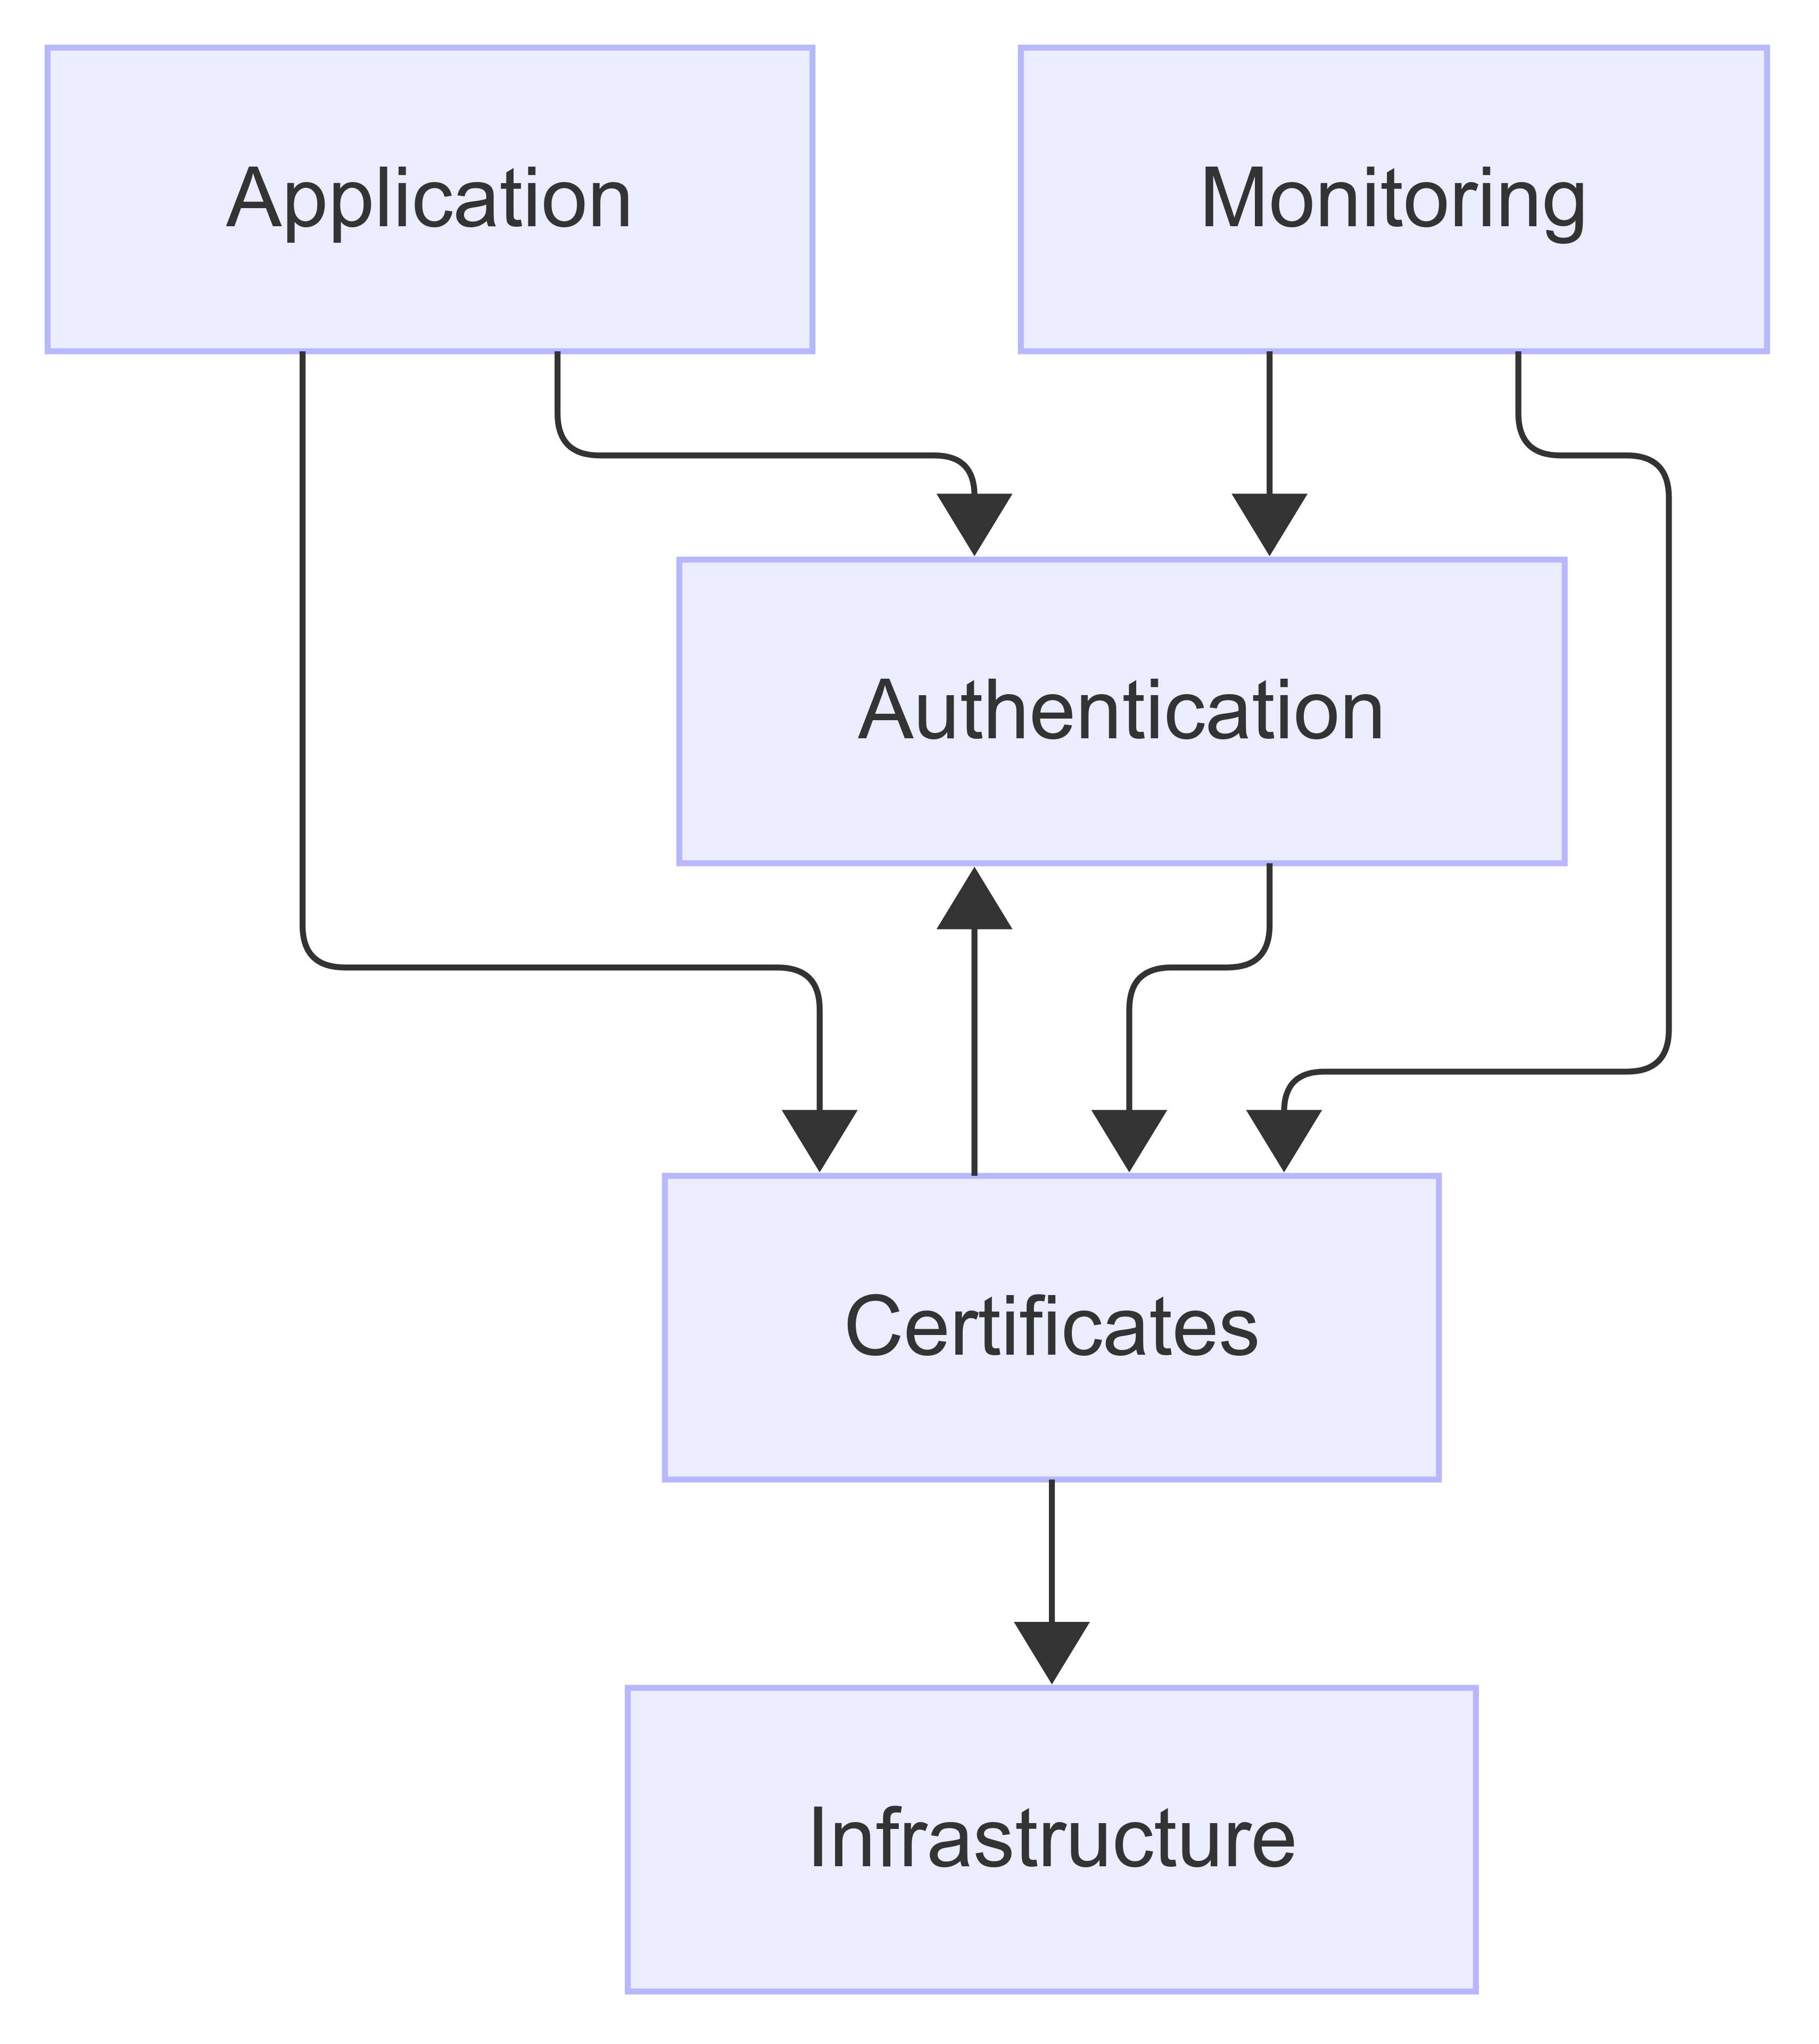
\includegraphics[width=.5\textwidth]{images/pulumi_stacks.png}
    \caption{Pulumi Stacks Relationship. An arrow pointing from a source to a target indicates that the source depends on the target. Given the layered approach, these relationships are transitive. However, arrows targeting certificates are explicitly included due to their significance.}
    \label{fig:pulumi_stacks}
\end{figure}

\section{Ansible}

\section{GitHub Actions}

\chapter{Cloud Agnostic Architecture}\label{chap:architecture}

\section{UCloud}

\section{Hetzner}

\section{Google}

\chapter{Dynamic Storage Provisioning}

\section{Rancher Local Path Provisioner}

\section{Network File System}

\section{File System in User Space}

\section{Object Storage}

\chapter{Private Key Infrastructure}

\section{Certificate Authority}

\section{Trust Chains}

\section{Certificate Signing Request}

\section{Smallstep}

\section{Let's Encrypt}

\section{TLS versus mTLS}

\section{SSH Certificate}

\section{Service Mesh}

\chapter{Identity \& Access Management}

\section{Realm \& Client}

\section{Token Claims \& Scopes}

\section{Supported Grant Types}

\chapter{Containers \& Virtual Machines}

\section{Docker in Docker}

\section{Kompose}

\section{KubeVirt}

\section{NixOS qcow2}

\chapter{Static Website}

\section{Jekyll}

\section{Home Page}

\section{GitHub Pages}

\chapter{CTFd}

\section{Authentication Plugin}

\section{Challenges Plugin}

\chapter{Deployer Service}

\section{Authentication}

\section{Networking}

\section{Deployment}

\section{Testing}

\section{Swagger}

\chapter{Feature Flag System}

\section{Strategies}

\section{Segments}

\chapter{Private Registry}

\section{htpasswd}

\section{Caching}

\section{Rate Limits}

\chapter{Monitoring}

\section{A Single Entry Point}

\section{Data Sources}

\section{Metric Collection}

\section{Logging}

\chapter{Static Code Analysis}

\section{SonarCloud}

\section{Dependabot}

\chapter{Evaluation}

\section{Qualitative Analysis}

\section{Quantitative Analysis}

\section{Feature Suggestions}

\chapter{Conclusion}

\cleardoublepage
\phantomsection
\addcontentsline{toc}{chapter}{References}
\printbibliography
\end{document}


\chapter{Kubernetes}

\section{Helm Chart}

\section{Horizontal Scaling}

\section{Vertical Scaling}

\section{Health Check}

\section{Probes}

\subsection{Liveness}

\subsection{Readiness}

\subsection{Statup}

\chapter{Development Environment}

\section{Automated Tasks}

\section{Domains}

\chapter{Infrastructure as Code}

\section{Pulumi}

\section{Alternatives}

\section{Developing a Provider}

\chapter{UCloud}

\section{Limited Network Access}

\section{Starting a Virtual Machine}

\section{Domain Name}

\chapter{Monitoring}
Monitoring is an essential aspect of managing a Kubernetes cluster. It provides a comprehensive overview of the health and performance of our services, enabling us to detect and address anomalies before they escalate into critical issues. Effective monitoring allows us to be proactive, ensuring the stability and reliability of our production environment. Rather than reacting to problems like firefighters, we aim to prevent issues from occurring in the first place.

In this chapter, we will explore the various technologies and tools used to achieve effective monitoring. Whether it involves sampling health metrics or gathering logs, the information should be accessible from a single entry point. Dashboards play a crucial role in this process, enhancing and contextualizing the data to make it meaningful and actionable. By leveraging these tools, we can maintain a robust and resilient Kubernetes cluster.

\section{A Single Entry Point}
Monitoring should be straightforward; otherwise, people will not use it! While the initial setup requires some effort, once it is running, all data should be readily available. Therefore, we want all our monitoring to be accessible from a single entry point, so that responsible personnel will not have to aggregate multiple sources to make a rational conclusion about the Kubernetes cluster’s health.

To achieve this single entry point, we will use the AIOps tool Grafana. Originally created as a fork of Kibana in 2014, Grafana has since specialized in integrating compatibility with multiple data sources, whereas Kibana is primarily compatible with Elasticsearch. Grafana's ability to support multiple data sources makes it a flexible and future-proof solution.

As a starting point, we will configure Prometheus, Loki, and possibly some databases as data sources. Prometheus is a time series database that collects various metrics. Loki is a system that collects and organizes log data for easy searching and viewing. The purpose of registering databases will primarily be for querying purposes, similar to tools like Adminer.

However, data sources alone will not suffice. As the name suggests, they are simply sources. The data needs to come from somewhere. Prometheus depends on Service Monitors or Pod Monitors to gather metrics, and Loki similarly relies on a log gatherer to collect and organize log data. Without these components, the data sources would remain empty and ineffective. Let us further explore the remaining tool stack in section \ref{sec:monitoring_stack}.

\section{The Technology Stack}\label{sec:monitoring_stack}
In this section, we will explore the use of tools developed by the Grafana and Prometheus community to monitor our Kubernetes cluster. To ensure comprehensive metric sampling, we will utilize various components to collect logs and scrape endpoints provided by the Kubernetes cluster. Below is an overview of the tools we will be using:

\begin{enumerate}
    \item \textbf{Promtail}: Promtail is an agent that ships the contents of local logs to a Loki instance. It is responsible for discovering targets, attaching labels, and pushing logs to the Loki instance.
    \item \textbf{Loki}: Loki is a horizontally-scalable, highly-available log aggregation system inspired by Prometheus. It is designed to be cost-effective and easy to operate, focusing on indexing metadata rather than the full text of the logs.
    \item \textbf{Prometheus}: Prometheus is an open-source systems monitoring and alerting toolkit. It collects and stores metrics as time series data, recording information with a timestamp.
    \item \textbf{Grafana}: Grafana is an open-source platform for monitoring and observability. It provides tools to query, visualize, alert on, and understand your metrics no matter where they are stored.
    \item \textbf{Component scraping the kubelet and kubelet-hosted cAdvisor}: This component scrapes metrics from the kubelet and cAdvisor, which provide information about the resource usage and performance of containers.
    \item \textbf{Component scraping the kube controller manager}: This component collects metrics from the Kubernetes controller manager, which manages the state of the cluster.
    \item \textbf{Component scraping CoreDNS or kubeDNS}: This component gathers metrics from CoreDNS or kubeDNS, which are responsible for DNS-based service discovery in the cluster.
    \item \textbf{Component scraping etcd}: This component scrapes metrics from etcd, the key-value store used as Kubernetes' backing store for all cluster data.
    \item \textbf{Component scraping the kube scheduler}: This component collects metrics from the Kubernetes scheduler, which assigns pods to nodes.
    \item \textbf{Component scraping the kube proxy}: This component gathers metrics from the kube proxy, which maintains network rules on nodes.
    \item \textbf{Component scraping kube state metrics}: This component collects metrics about the state of the Kubernetes objects, such as deployments, nodes, and pods.
    \item \textbf{Deploy node exporter as a daemonset to all nodes}: Node exporter runs on each node to expose hardware and OS metrics.
    \item \textbf{Prometheus Operator}: The Prometheus Operator simplifies the deployment and management of Prometheus and related monitoring components.
\end{enumerate}

The scraping components consist of a service, an associated service monitor, and in some cases, an Endpoints resource. These components are crucial for gathering metrics from various parts of the Kubernetes cluster.

To ensure comprehensive monitoring, we employ both active (intrusive) and passive (non-intrusive) monitoring techniques. Active monitoring involves modifying code to record specific metrics and send information to a logging system, which provides detailed, application-specific insights but adds some overhead. Passive monitoring, on the other hand, collects metrics from the system running the container or VM without modifying the application, offering a broader but more generic view. An example of intrusive monitoring is the metrics endpoint on Loki or Prometheus, while passive monitoring is exemplified by the CAdvisor integrated into the Kubelet, which monitors container resource usage without the containers being aware. By combining both methods, we achieve a balanced and effective monitoring strategy.

As mentioned in the introduction, we have decided to rely primarily on Helm charts when possible. Grafana and Prometheus provide and maintain excellent Helm charts that include features such as horizontal scaling, network policies, and cluster roles. These resources would be complex to create ourselves, so it is beneficial to leverage these pre-built charts.

However, Helm charts are designed to bundle resources, which raises the question of what should be bundled together. For instance, if Grafana is included in multiple Helm charts, which chart should be responsible for deploying it? In this project, we have decided that Helm charts should be as minimal as possible. If it is straightforward to create the integrations ourselves, that is our preferred approach. Helm charts created for specific services, rather than large bundles, are usually easier to configure and comprehend. Moreover, Helm charts targeting deeper integrations align better with our goal of low coupling and high cohesion. Being less dependent on complex charts makes it easier to add or remove services later, allowing us to stay agile and less committed to existing developments.

We utilized several Helm charts to streamline the deployment and management of our monitoring tools. From the Grafana Helm chart repository (\url{https://grafana.github.io/helm-charts}), we used the charts for Grafana, Loki, and Promtail. Additionally, from the Prometheus Community Helm chart repository (\url{https://prometheus-community.github.io/helm-charts}), we employed the kube-prometheus-stack chart.

While considering log shipping solutions, we evaluated both Promtail and Fluent Bit. Promtail is known for its seamless integration with Loki, making it an ideal choice for Kubernetes environments. On the other hand, Fluent Bit offers high performance and flexibility, capable of forwarding logs to multiple destinations. Ultimately, we chose Promtail for its simplicity and compatibility within the Loki ecosystem, which aligns with our goal of maintaining a cohesive and efficient monitoring setup.

\section{Sidecar Container}
In Kubernetes, sidecar containers are a design pattern where an additional container runs alongside the main application container within the same pod. This pattern extends the functionality of the main application without modifying its code. A common use case for sidecar containers is dynamically loading dashboards into Grafana. This approach is particularly advantageous because it avoids unnecessary rolling updates of Grafana, making it super easy to configure new dashboard resources. For example, if using an external Helm chart with their own custom dashboards for Grafana, made for their service, then the dashboards are easily deployed, as there is no need to change the configuration of the currently running Grafana instance. To achieve this, \texttt{ConfigMaps} containing the dashboards must be labeled appropriately, such as with the label \texttt{grafana\_dashboard}. These \texttt{ConfigMaps} should include key-value pairs where the key is the filename and the value is the JSON content of the dashboard.

The sidecar container used for this purpose is typically based on a general-purpose image like \texttt{kiwigrid/k8s-sidecar}. This container continuously scans for \texttt{ConfigMaps} with the specified label and loads them into Grafana using Grafana's public API. The sidecar container is configured with environment variables that specify how to interact with Grafana, including the Grafana URL and an API key for authentication. The API key is usually stored in a Kubernetes Secret and mounted into the sidecar container.

The sidecar container works by continuously scanning the Kubernetes API for \texttt{ConfigMaps} labeled with \texttt{grafana\_dashboard}. When it detects a \texttt{ConfigMap} with this label, it reads the JSON content and stores it in a specified folder within the pod. The sidecar then uses Grafana's public API to import the dashboards, ensuring that any new or updated dashboards are automatically loaded into Grafana without manual intervention. This approach allows for dynamic management of Grafana dashboards, making it easier to update and maintain them as part of a Kubernetes deployment.

Similar features have been prepared for automatically adding scraping targets to Prometheus. These are known as Service Monitors or Pod Monitors, which will be described in the following two sections.

\section{Custom Resource Definition}
In Kubernetes, when the default resources do not meet specific requirements, it is possible to define custom resources to extend the functionality of the cluster. This capability is leveraged by the Prometheus community to introduce a set of Custom Resource Definitions (CRDs) that facilitate advanced monitoring configurations. These CRDs enable the seamless integration and management of Prometheus and related components within a Kubernetes environment. Although not all CRDs are utilized in every deployment, they are included due to their lightweight nature and the complexity involved in selectively disabling them. The Helm chart containing these CRDs is part of the kube-prometheus-stack.

The primary CRDs introduced by the Prometheus community include:

\begin{enumerate}
    \item \textbf{Prometheus}: Defines a Prometheus instance, allowing configuration of replicas, persistent storage, and alerting mechanisms.
    \item \textbf{Alertmanager}: Manages \texttt{Alertmanager} instances, which handle alerts sent by Prometheus and support high availability configurations.
    \item \textbf{ThanosRuler}: Sets up Thanos Ruler instances for processing recording and alerting rules across multiple Prometheus instances.
    \item \textbf{ServiceMonitor}: Specifies how a set of services should be monitored, including endpoints and scraping intervals.
    \item \textbf{PodMonitor}: Similar to \texttt{ServiceMonitor}, but specifically targets pods for monitoring.
    \item \textbf{Probe}: Defines blackbox probing configurations to monitor endpoints from an external perspective.
    \item \textbf{PrometheusRule}: Manages Prometheus recording and alerting rules.
    \item \textbf{AlertmanagerConfig}: Configures \texttt{Alertmanager} settings, such as routing and notification templates.
    \item \textbf{PrometheusAgent}: Sets up a lightweight Prometheus Agent instance for scraping and forwarding metrics.
    \item \textbf{ScrapeConfig}: Provides additional scraping configurations for Prometheus instances.
\end{enumerate}

The Prometheus Operator periodically scans for \texttt{ServiceMonitors}, which define how services should be monitored. Upon discovery, the operator updates Prometheus with the new scraping targets. This allows services exposing metrics in a text-based exposition format to be dynamically added to Prometheus without modifying its configuration or triggering a rolling update. This approach enhances flexibility and reduces operational overhead in maintaining the monitoring setup.

These CRDs facilitate the Kubernetes-native deployment and management of Prometheus and its ecosystem, streamlining the setup and maintenance of an effective monitoring stack.

Deploying the kube-prometheus-stack with Pulumi can sometimes result in failures when resources using a CRD type are detected before the CRD is created. Pulumi may mark these resources as failed after several attempts, an issue that does not occur with Helm. To mitigate this, we take advantage of the Helm chart's design, which allows individual components to be toggled. The CRDs are deactivated as part of the monitoring project but created as part of the fundamental configuration of the Kubernetes cluster.

\section{Service Monitor}
This section will delve into the definition and use of \texttt{ServiceMonitor}, while also comparing it with \texttt{PodMonitor}.

A \texttt{ServiceMonitor} is a CRD that specifies how groups of services should be monitored. It allows Prometheus to scrape metrics from services by defining endpoints and selectors. Here is an example of how to define a \texttt{ServiceMonitor} using TypeScript:

\begin{minted}{typescript}
new k8s.apiextensions.CustomResource("<resource>", {
    apiVersion: "monitoring.coreos.com/v1",
    kind: "ServiceMonitor",
    metadata: {
        namespace: "<namespace>",
        labels: {
            release: "<releaseName>"
        }
    },
    spec: {
        endpoints: [{
            interval: "30s",
            port: "<DNSLabel>"
        }],
        selector: {
            matchLabels: appLabels
        }
    }
})
\end{minted}

In this example, the \texttt{ServiceMonitor} is configured to scrape metrics every 30 seconds from a specified port. The \texttt{selector} field uses labels to identify the services to monitor.

When defining Service Monitors, it is crucial to consider the release label. The Prometheus Operator will only discover Service Monitors or Pod Monitors that are within its release. Additionally, by default, the Prometheus Operator is configured to discover monitors across all namespaces. However, the Prometheus instance itself will, by default, only add scraping targets for monitors that reside within its own namespace.

When defining endpoints in a \texttt{ServiceMonitor}, you can specify either \texttt{port} or \texttt{targetPort}. The \texttt{port} must be a DNS label string referring to a named port defined in a service, while \texttt{targetPort} can be an integer or string representing the target port of the \texttt{Pod} object\footnote{The port must be specified with the container's port property.} behind the service.

While \texttt{ServiceMonitor} is used to monitor services, \texttt{PodMonitor} is designed to monitor pods. Here are the key differences:

\begin{itemize}
    \item \textbf{ServiceMonitor}: Ideal for monitoring a group of pods behind a service. It simplifies the configuration by using service labels and is useful when you want to get a collective measure of the pods running behind a service.
    \item \textbf{PodMonitor}: Suitable for monitoring individual pods directly. It is useful when you need to scrape metrics from specific pods without defining a service. For example, monitoring SQL exporters where you want to consistently scrape each pod's \texttt{/metrics} endpoint without being challenged by load balancing.
\end{itemize}

In summary, use \texttt{ServiceMonitor} when you have services managing multiple pods and need aggregated metrics. Use \texttt{PodMonitor} when you need detailed metrics from individual pods, especially when services are not defined or needed. Everything mentioned in this section has been tested through an experiment.

\chapter{Identity \& Access Management}
In today's digital landscape, software platforms must support a diverse array of users, each with distinct organizational roles and access rights. This is particularly crucial when developing a CTF platform, where managing user authentication and authorization becomes essential. Authentication verifies a user's identity, while authorization determines their access rights.

A key decision in Identity and Access Management (IAM) is whether to adopt a centralized or decentralized approach. Centralized IAM simplifies management by consolidating user data and access controls in one place, making it easier for administrators to configure and maintain. This approach also facilitates Single Sign-On (SSO), allowing users to authenticate once and gain access to multiple services.

On the other hand, decentralized IAM, though more complex to develop, offers significant benefits. It distributes authentication and authorization responsibilities across various services, enhancing security and resilience. Fortunately, open-source solutions implementing standardized protocols can handle these complexities, providing robust IAM capabilities without the need for extensive in-house development.

By leveraging these solutions, organizations can ensure secure, efficient, and scalable management of user identities and access rights, ultimately enhancing the overall user experience and system security.

For this project, we decided to use the multi-tenant open-source service named Keycloak \parencite{keycloak}. The choice was not based on academic reasons but rather on prior experience configuring this service. Several alternatives could have been considered, such as Zitadel, Apereo CAS, LemonLDAP::NG, and Gluu Server. These services support the same protocols, with some exceptions: Gluu Server also supports SCIM, while Zitadel does not support SAML. 

It is important to mention that for configuring external authentication on Grafana, we rely on Generic OAuth. This protocol is only surpassed by LDAP in terms of preference \parencite{grafana_authentication}. Further investigation led us to an article by Grafana, which directly recommends Keycloak as an OAuth2 provider, highlighting it as the only open-source service on the list \parencite{grafana_oauth}. This confirms that Keycloak is a sufficient and reliable solution for our needs.

\section{Protocols}
\todo{Study this}

\section{Realm \& Client}
When deploying Keycloak, we rely on a Helm chart maintained by Bitnami \parencite{bitnami_keycloak}. Keycloak's documentation can be challenging to navigate, making it difficult to compare the Helm chart with the official documentation to determine how to fill in the Helm \texttt{values.yaml} file. However, after some effort, we managed to configure it. This configuration is part of the monitoring Pulumi project. More interesting is how to configure Keycloak itself to ensure reliable integrations with other services.

The fundamental pillars consist of configuring the realm and corresponding clients. First, what is a realm? A realm is a fundamental concept used to manage a set of users, credentials, roles, and groups. Realms offer isolation, as each realm is independent of others, meaning users, roles, and configurations in one realm do not affect those in another. This isolation enables multi-tenancy, allowing different organizations or projects to use the same Keycloak instance without interfering with each other. Each realm can be configured to use its own identity providers, user federations, authentication flows, and more. Our CTF platform only has a single tenant, so one realm is sufficient. Let's call this realm \texttt{CTF} for clarity.

Next, what is a client? The answer is simple when thinking about typical server-client communication. The server (Keycloak) receives requests from clients (services). It is good practice to create a client for each service using Keycloak. This approach allows for configuring allowed hosts, allowed redirects, and each client having its own client secret (if enabled). This ensures that no clients can conflict, as only the client that should be able to make requests would have the secret to do so. The default settings should be sufficient, as we intend to rely on the access token and foresee the ID token -- more on this in section \ref{sec:token_claims}.

When the realm and clients have been configured, we will need to export the configuration so that it can be stored statically and loaded dynamically when needed. The realm and client settings should not be lost just because the Kubernetes cluster is reset!

\todo{Generating the client secret?}

\section{Token Claims \& Scopes}\label{sec:token_claims}
Authenticating using Keycloak will return a JWT in response. This JWT contains both an ID token and an access token. The access token can be used to query the userinfo endpoint if needed. The content or claims within the JWT must be configured in Keycloak. This project uses the default settings, which already provide the necessary information in the access token. However, if roles are needed in either the userinfo or the ID token, a predefined mapper must be configured to include these claims. The access- and ID token is by default encoded using the RS256 algorithm -- RSA Digital Signature Algorithm with the SHA-256 hash function.

The JWT includes some default metadata claims that provide information about who issued the token, when it was issued, and other essential details. The mandatory claims are listed below:

\begin{itemize} 
    \item \textbf{iss (Issuer)}: Identifies the principal that issued the JWT.
    \item \textbf{aud (Audience)}: Identifies the recipients that the JWT is intended for. 
    \item \textbf{exp (Expiration Time)}: Identifies the expiration time on or after which the JWT must not be accepted for processing. 
    \item \textbf{iat (Issued At)}: Identifies the time at which the JWT was issued. 
    \item \textbf{jti (JWT ID)}: Provides a unique identifier for the JWT, which can be used to prevent the JWT from being replayed. 
\end{itemize}

Keycloak includes certain scopes by default without needing to request them explicitly. Each scope can encompass multiple claims, and the descriptions below provide an idea of what those claims might include:

\begin{itemize} 
    \item \textbf{acr}: The Authentication Context Class Reference, indicating the level or method of authentication. 
    \item \textbf{basic}: Typically includes basic user information such as user ID (the \texttt{sub} claim) and authentication time. 
    \item \textbf{email}: Contains the user's email address and a flag indicating whether the email has been verified. 
    \item 
    \textbf{profile}: Includes profile information such as name, family name, given name, nickname, and profile picture. 
    \item \textbf{roles}: Lists the roles assigned to the user, which can be used for authorization purposes. 
\end{itemize}

There are also scopes that must be explicitly requested. This includes information like address and phone number, which are not included by default to protect user privacy:

\begin{itemize} 
    \item \textbf{address}: Contains the user's address information. 
    \item \textbf{microprofile-jwt}: A claim used in MicroProfile JWT for additional JWT token information. 
    \item \textbf{offline\_access}: Indicates that the token can be used to obtain a refresh token for offline access. 
    \item \textbf{phone}: Includes the user's phone number and a flag indicating whether the phone number has been verified. 
\end{itemize}

Being aware of the JWT's content is definitely useful, as will become evident when discussing some of the difficulties that arose when configuring Grafana to use Keycloak for authentication, as detailed in section \ref{sec:grafana_auth}.

\section{Supported Grant Types}
Keycloak supports various OAuth 2.0 grant types to cater to different authentication scenarios. These grant types define the methods through which clients can obtain access tokens, each suited for specific use-cases and accompanied by unique security considerations.

The information presented in this section is based on the official Keycloak documentation, which provides comprehensive details on the supported grant types and their respective use-cases and security considerations \Parencite{keycloak2024}.

\subsection*{Authorization Code}\label{sec:auth_code}
The Authorization Code Grant is primarily used by web and mobile applications. It involves a two-step process where the client first obtains an authorization code, which is then exchanged for an access token. This method ensures that the client never directly handles the user's credentials, enhancing security by reducing the risk of credential exposure.

A diagram showing the flow is given below:

\begin{tcolorbox}
\begin{scriptsize}
\begin{verbatim}
            +----------+
            | Resource |
            |   Owner  |
            +----------+
                 ^
                 |
                (B)
            +----|-----+          Client Identifier      +---------------+
            |         -+----(A)-- & Redirection URI ---->|               |
            |  User-   |                                 | Authorization |
            |  Agent  -+----(B)-- User authenticates --->|     Server    |
            |          |                                 |               |
            |         -+----(C)-- Authorization Code ---<|               |
            +-|----|---+                                 +---------------+
              |    |                                         ^      v
             (A)  (C)                                        |      |
              |    |                                         |      |
              ^    v                                         |      |
            +---------+                                      |      |
            |         |>---(D)-- Authorization Code ---------'      |
            |  Client |          & Redirection URI                  |
            |         |                                             |
            |         |<---(E)----- Access Token -------------------'
            +---------+       (w/ Optional Refresh Token)

        Note: The lines illustrating steps (A), (B), and (C) are broken into
        two parts as they pass through the user-agent.

                            Authorization Code Flow

        https://datatracker.ietf.org/doc/html/rfc6749#section-4.1
\end{verbatim}
\end{scriptsize}
\end{tcolorbox}

This two-step process is essential for avoiding issues with Cross-Origin Resource Sharing (CORS). CORS is a security feature implemented by web browsers to prevent web pages from making requests to a different domain than the one that served the web page, known as the same-origin policy. By using the Authorization Code Grant, the exchange of the authorization code for an access token happens server-to-server, reducing the risk of exposing sensitive information through client-side scripts, which could be subject to CORS restrictions.

\subsection*{Implicit}
The Implicit Grant is designed for browser-based applications like single-page applications (SPAs). In this flow, the access token is issued directly without an intermediate authorization code. A key security risk is that the token is provided in the URL, which can be logged in browser history, server logs, or shared inadvertently, exposing the token to malicious actors. On the positive side, the client does not handle user credentials directly.\todo{revise SPA}

Including the access token in the URL is necessary to address CORS restrictions. CORS policies can block requests from the browser to a different domain if the access token is included in the response body, as this can trigger a preflight request.

To mitigate these risks, the token is short-lived, minimizing the window for misuse. This flow is used for quick authentication, where the token is used briefly and then discarded. Additionally, the Implicit Grant does not provide a refresh token, as these are long-lived and pose a significant security risk if exposed. By not issuing a refresh token, the access token's lifespan is limited, reducing the impact of potential interception.

According to the current OAuth 2.0 Security Best Current Practice, the Implicit Grant flow is discouraged due to its security vulnerabilities. Consequently, this flow has been removed from the upcoming OAuth 2.1 specification.

\subsection*{Resource Owner Password Credentials}
The Resource Owner Password Credentials (ROPC) Grant is intended for scenarios where the user has a high level of trust in the client application, such as first-party clients. In this flow, the client application directly collects the user's credentials (username and password) and exchanges them for an access token from the authorization server. This method is straightforward but comes with significant security risks, as the client handles the user's credentials directly.

A major drawback of the ROPC Grant is the potential exposure of user credentials. If the client application is compromised, the user's credentials can be intercepted and misused. Additionally, this flow does not support multi-factor authentication (MFA), which further reduces its security robustness.

Despite these risks, the ROPC Grant can be useful in specific cases, such as when migrating legacy applications that already collect user credentials. It allows these applications to transition to OAuth 2.0 without requiring significant changes to their authentication mechanisms.

The OAuth 2.0 Security Best Current Practice advises against using the ROPC Grant due to its inherent vulnerabilities. As a result, this flow is being deprecated in favor of more secure alternatives like the Authorization Code Grant.

\subsection*{Client Credentials}
The Client Credentials Grant is used when clients (applications and services) need to obtain access on behalf of themselves rather than on behalf of a user. This flow is particularly useful for background services that apply changes to the system in general rather than for a specific user. In this flow, the client application authenticates with the authorization server using its client credentials (client ID and client secret) and directly obtains an access token.

Keycloak supports client authentication using either a secret or public/private keys. This flexibility allows for secure authentication methods tailored to the specific needs of the client application.

One of the main advantages of the Client Credentials Grant is its simplicity and efficiency in scenarios where user context is not required. However, it also means that the access token obtained is limited to the permissions granted to the client application itself, rather than any specific user.

\subsection*{Device Authorization Grant}
The Device Authorization Grant is used by clients running on internet-connected devices that have limited input capabilities or lack a suitable browser, such as smart TVs, gaming consoles, or IoT devices. In this flow, the application requests that Keycloak provide a device code and a user code. Keycloak creates these codes and returns them to the application.

The application then provides the user with the user code and a verification URI. The user accesses this verification URI on another device with a suitable browser to authenticate. Meanwhile, the application repeatedly polls Keycloak until the user completes the authorization process.

Once user authentication is complete, the application obtains the device code. The application then uses this device code along with its credentials to obtain an Access Token, Refresh Token, and ID Token from Keycloak.

This grant type is particularly useful for scenarios where user interaction with the device is limited or cumbersome. It allows the user to authenticate on a more convenient device, such as a smartphone or computer, while the original device remains in a waiting state.

\subsection*{Client Initiated Backchannel Authentication Grant}
The Client Initiated Backchannel Authentication (CIBA) Grant is used by clients to initiate the authentication flow without redirecting through the user's browser. This is particularly useful for devices with limited input capabilities, such as smart TVs or IoT devices. The app requests an \texttt{auth\_req\_id} from Keycloak, and the user completes authentication on a separate device. This flow allows for secure login without direct user interaction with the app.

\newpage

\section{Integrations}
The significance of Keycloak lies in its practical application. In the following sections, we will explore how Keycloak plays a crucial role in managing authentication for our services. Some open-source software, such as Grafana, allows for seamless integration with Keycloak, making the process straightforward. In contrast, other software solutions, like CTFd, require more effort to integrate. The specifics of these integrations will be detailed in the associated sections.

\subsection{CTFd}
CTFd is arguably our most important exposed service from a practical user perspective. As a web-based platform designed to host CTF competitions, it requires an efficient way to manage users. Ideally, we would leverage external identity providers to avoid the hassle of user creation, relying instead on higher-level institutions or organizations to provide these identities.

However, there is a significant challenge: CTFd does not support any form of SSO unless it is either an enterprise or hosted version \parencite{ctfd_sso}. This limitation forces us to make a choice. Given that CTFd is open-source, we can either 1) modify the source code to implement SSO our way, or 2) create a custom plugin to handle authentication. Modifying the source code would necessitate freezing the version, as future updates could disrupt our changes. Therefore, creating a plugin is the more rational approach.

Fortunately, creating plugins for CTFd is relatively straightforward and well-documented \parencite{ctfd_plugins}. However, there is a notable issue with how the Docker image is developed. Plugin requirements are installed at build time rather than at the entrypoint, which complicates the process. This means we cannot simply mount the plugin to the specified folder without building the Docker file from scratch, as the necessary pip packages are not installed. The solution was to update the entrypoint -- a simple but inconvenient fix\todo{revise}.

The most important detail about the Keycloak plugin developed for CTFd is that it can be configured using the \texttt{config.json} file, and that endpoints can be overwritten as follows:

\begin{minted}{py3}
app.view_functions['auth.login'] = lambda: redirect(url_for('keycloak'))
app.view_functions['auth.logout'] = lambda: redirect(url_for('keycloak_logout'))
app.view_functions['auth.register'] = lambda: ('', 204)
app.view_functions['auth.reset_password'] = lambda: ('', 204)
app.view_functions['auth.confirm'] = lambda: ('', 204)
\end{minted}

When the user clicks the login button, they are redirected to our custom login page instead of the usual login page. The same applies to the logout button. Additionally, endpoints can be disabled in this manner, resulting in a 204 status code (indicating that the request has been successfully processed, but no content is returned). The code block above demonstrates that if the register button is made public during setup, it will not function as it redirects to nowhere. The same logic applies to the reset password and confirm (login callback) endpoints.

The implementation has been done using \texttt{python-keycloak} \parencite{python_keycloak}, a tool specialized for handling authentication with Keycloak, utilizing the \textit{authorization code} grant type. While a more general approach could have involved using a generic OIDC plugin, \texttt{python-keycloak} was chosen for its ease of use and effectiveness in solving our specific problem.

The login flow utilizes the Authorization Code Grant (see Section \ref{sec:auth_code}) and operates as follows:

\begin{enumerate}
    \item A user logs into CTFd using their SSO credentials.
    \item If the user does not exist in CTFd's database, they are created; otherwise, the existing user is fetched.
    \item Roles and other profile settings are synchronized to match the configurations of the SSO user.
    \item The user is then logged into CTFd with their SSO credentials.
\end{enumerate}

If necessary, administrators can disable or ban users from CTFd. It is important to note that even if a user is deleted from CTFd's database, they will be recreated upon logging in again. Conversely, if a user is deleted in Keycloak, they will still exist in CTFd's database but will be unable to log in, as authentication is handled by Keycloak. Therefore, to properly delete a user, they must be removed from both databases, or at least from CTFd's database with their roles revoked to prevent authorization upon authentication.

In SQLAlchemy, \texttt{polymorphic\_on} and \texttt{polymorphic\_identity} are used to handle inheritance in database models. The \texttt{polymorphic\_on} attribute specifies the column used to determine the type of the object, while \texttt{polymorphic\_identity} sets the identity for each subclass. This allows SQLAlchemy to distinguish between different types of objects stored in the same table.

\begin{minted}{py3}
class Users(db.Model):
    __tablename__ = "users"
    __mapper_args__ = {"polymorphic_identity": "user", "polymorphic_on": type}
    ...

class Admins(Users):
    __tablename__ = "admins"
    __mapper_args__ = {"polymorphic_identity": "admin"}
\end{minted}

The \texttt{Submissions} class has a foreign key \texttt{user\_id} that references the \texttt{users} table. The \texttt{ondelete="CASCADE"} ensures that when a user is deleted, all related submissions are also deleted.

\begin{minted}{py3}
class Submissions(db.Model):
    __tablename__ = "submissions"
    id = db.Column(db.Integer, primary_key=True)
    user_id = db.Column(db.Integer, db.ForeignKey("users.id", ondelete="CASCADE"))
\end{minted}

Handling polymorphic types can be challenging, especially when changing the type of an existing object. For example, if you add an admin and later change its type to user, you might encounter an \texttt{ObjectDeletedError}. This error occurs because changing the polymorphic identity can lead to the deletion of the original object, causing issues with related objects like submissions and comments that are linked via foreign keys with cascade delete.

To handle the issue of changing polymorphic types without losing related objects, you can generate the response first before actually changing the type. This avoids the \texttt{ObjectDeletedError}. This solution was found by reading through the source code for CTFd's public API \cite{CTFdUsersAPI}.

\begin{minted}{py3}
def patch_user(user_id, data):
    user = Users.query.filter_by(id=user_id).first_or_404()
    data["id"] = user_id

    schema = UserSchema(view="admin", instance=user, partial=True)
    response = schema.load(data)
    if response.errors:
        return {"success": False, "errors": response.errors}, 400

    # This generates the response first before actually changing the type
    # This avoids an error during User type changes where we change
    # the polymorphic identity resulting in an ObjectDeletedError
    # https://github.com/CTFd/CTFd/issues/1794
    response = schema.dump(response.data)
    ...
\end{minted}

By understanding and properly handling polymorphic types in SQLAlchemy, you can avoid issues like \texttt{ObjectDeletedError} and ensure that related objects are preserved when changing the type of a user. This involves generating responses before changing types and using methods to manage related objects effectively. This approach ensures that properties and linked objects like submissions and comments are not lost during the type change.\todo{explain API keys}

\subsection{Grafana}\label{sec:grafana_auth}
Integrating Grafana with Keycloak addresses the critical challenges of secure and efficient user authentication and authorization by leveraging standardized protocols. This section details the configuration process, focusing on protocol integration, PKCE, refresh tokens, role mapping, and the underlying protocols \parencite{GrafanaKeycloak}.

\begin{minted}{javascript}
{
    "auth.generic_oauth": {
        enabled: true,
        use_pkce: true,
        allow_sign_up: true,
        use_refresh_token: true,
        role_attribute_strict: true,
        client_secret: GRAFANA_CLIENT_SECRET,
        scopes: "openid",
        client_id: "grafana",
        name: "Keycloak-OAuth",
        name_attribute_path: "name",
        email_attribute_path: "email",
        id_token_attribute_name: "access_token",
        login_attribute_path: "preferred_username",
        token_url: `${keycloakIntern}/realms/ctf/protocol/openid-connect/token`,
        auth_url: `${keycloakExtern}/realms/ctf/protocol/openid-connect/auth`,
        api_url: `${keycloakExtern}/realms/ctf/protocol/openid-connect/userinfo`,
        signout_redirect_url: `${keycloakExtern}/realms/ctf/protocol/openid-connect/logout`,
        role_attribute_path: "contains(resource_access.grafana.roles, 'admin') && 'Admin' || contains(resource_access.grafana.roles, 'editor') && 'Editor' || ''"
    }
}
\end{minted}

Grafana integrates with Keycloak using OAuth2 and OIDC. Key endpoints include the authorization endpoint, token endpoint, user info endpoint, and logout endpoint. By setting \texttt{id\_token\_attribute\_name} to \texttt{access\_token}, Grafana uses the access token for authorization, avoiding the need for additional client mappers required by the ID token used by default; otherwise, Grafana will not be able to find the client roles. This approach simplifies the configuration by utilizing the readily available information already in the access token.

Grafana uses the \texttt{sub} claim as the unique identifier for the user. This can be changed to the email by setting \texttt{oauth\_allow\_insecure\_email\_lookup} to \texttt{true}. This option is typically used when authenticating with different identity providers. However, it is noteworthy that user synchronization issues may arise if the basic claim scope is missing \parencite{grafana_authentication}.

PKCE enhances the security of the OAuth2 authorization code flow, particularly for public clients. It mitigates authorization code interception attacks by introducing a code verifier and code challenge. The client generates a code verifier and sends a hashed code challenge to the authorization server. Upon exchanging the authorization code for an access token, the client presents the original code verifier. This ensures that intercepted authorization codes cannot be used without the code verifier, significantly enhancing security.

Refresh tokens maintain user sessions without frequent re-authentication. Upon initial login, both an access token and a refresh token are issued. The access token has a short lifespan, while the refresh token is long-lived. When the access token expires, the client uses the refresh token to obtain a new access token, ensuring continuous access and improving user experience while maintaining security.

Role mapping in Grafana is achieved using JMESPath, a query language for JSON. The \texttt{role\_attribute\_path} configuration extracts and maps roles from the Keycloak token to Grafana roles. This path dynamically maps Keycloak roles to Grafana roles, ensuring accurate user permissions.

Integrating Grafana with Keycloak for authentication provides a secure and efficient solution for managing user access in modern web applications. By leveraging OAuth2 and OIDC protocols, utilizing PKCE, implementing refresh tokens, and employing dynamic role mapping, this integration enhances security and user experience, ensuring that only authorized users can access sensitive data visualized in Grafana.

\subsection{Step Certificates}

\subsection{APIs}

\chapter{Certificate Management}

It’s both. The CRD (Custom Resource Definition) StepIssuer defines how cert-manager interacts with the step issuer, and using cert-manager.io/v1 as the API version ensures that cert-manager processes the certificate request.

The StepIssuer CRD is what allows cert-manager to understand and utilize Step Issuer-specific configurations. The apiVersion specifies that this CRD is part of cert-manager’s ecosystem, linking the certificate management workflow to the Step Issuer capabilities.

So, it’s the combination of the StepIssuer CRD defining the step-issuer's specifics and the API version that ties it into cert-manager’s functionality.

\section{Zero Trust}

\section{Certificate Authority}

\section{ACME for TLS}

\section{SSH Certificates}

\section{Smallstep}

\subsection{Smallstep SSH}

\subsection{Step Certificates}

\subsection{Autocert}

\subsection{Issuer}

\subsection{Bootstrap}

\begin{minted}{bash}
fingerprint=$(
    curl -k https://myhost/roots.pem | 
    openssl x509 -noout -sha256 -fingerprint | 
    sed 's/://g' | 
    tr 'A-F' 'a-f' | 
    awk -F= '{print $2}'
)

step ca bootstrap --ca-url https://myhost \
    --fingerprint $fingerprint \
    --force \
    --install
\end{minted}


% https://github.com/smallstep/cli/blob/3d38cfeadb8f90e8b916a7b7e9c1d4fe9e80a43f/command/oauth/cmd.go#L331

% step will expect to be able to perform a TLS handshake with the proxy, and use the CA's root certificate to complete the trust chain. So, for inbound TLS connections, the proxy should use a server certificate issued by step-ca. See below for an example.

% Layer 4 (Transport Layer): This deals with transportation of data between systems. It doesn’t concern itself with what the data is, but with the movement of the data packets. In a layer 4 proxy, this means forwarding traffic based purely on TCP/UDP protocols without looking at the actual content. This is often referred to as "TLS passthrough" because the proxy doesn’t terminate the SSL/TLS connection—it just passes it through to the backend server.

% Layer 7 (Application Layer): This goes a step further, inspecting and potentially modifying the data itself because it operates at the application level. A layer 7 proxy can make decisions based on HTTP headers, cookies, and other data in the web traffic, allowing for more sophisticated routing and filtering. The proxy terminates the SSL/TLS connection, decrypts the data, and then possibly re-encrypts it before sending it to the backend server.

% Layer 1 - Physical: Deals with the physical connection between devices, including cables and switches.

% Layer 2 - Data Link: Manages data transfer between adjacent network nodes, using MAC addresses.

% Layer 3 - Network: Handles routing of data packets using IP addresses.

% Layer 4 - Transport: Ensures reliable data transfer with error correction and flow control (e.g., TCP/UDP).

% Layer 5 - Session: Manages sessions or connections between applications.

% Layer 6 - Presentation: Translates data between the application layer and the network, dealing with data encryption and compression.

% Layer 7 - Application: Provides network services directly to end-user applications, such as web browsers and email clients.

% The Root function in the step-ca client code requires no TLS termination because it relies on a direct, secure connection to the CA to ensure the integrity and authenticity of the root certificate. Here’s a detailed explanation:

% Key Points of the Root Function
% Direct HTTPS Request:
% Go

% resp, err := c.httpClient.Get(c.baseURL + "/root/" + fingerprint)
% Kode genereret af kunstig intelligens. Gennemse og brug forsigtigt. Flere oplysninger om ofte stillede spørgsmål.
% This line makes an HTTPS request to the CA to retrieve the root certificate. The httpClient is configured to establish a secure TLS connection directly to the CA.
% Certificate Validation:
% Go

% defer resp.Body.Close()
% // Parse and validate the certificate
% Kode genereret af kunstig intelligens. Gennemse og brug forsigtigt. Flere oplysninger om ofte stillede spørgsmål.
% After receiving the response, the function parses and validates the certificate. This validation process ensures that the certificate matches the expected fingerprint and is trusted.
% Why No TLS Termination is Required
% End-to-End Encryption:
% The Root function expects the entire communication path to be encrypted from the client to the CA. TLS termination at the ingress would break this end-to-end encryption, as the ingress would decrypt and then re-encrypt the traffic. This intermediate step can introduce security risks and prevent the client from validating the CA’s certificate directly.
% Certificate Integrity:
% The client needs to ensure that the root certificate it receives is authentic and has not been tampered with. By maintaining a direct TLS connection, the client can securely retrieve and validate the certificate against the provided fingerprint. Any interruption in this secure channel could compromise the integrity of the certificate.
% Security Policies:
% The step CLI and step-ca are designed with strict security policies that require direct, secure communication with the CA. Allowing TLS termination would violate these policies and potentially expose the communication to man-in-the-middle attacks.
% Summary
% In summary, the Root function requires a direct, uninterrupted TLS connection to ensure the security and integrity of the root certificate retrieval process. SSL passthrough is necessary to maintain this secure connection from the client to the CA, preventing any intermediate decryption and re-encryption that could compromise the security.

% // BootstrapClient is a helper function that using the given bootstrap token
% // return an http.Client configured with a Transport prepared to do TLS
% // connections using the client certificate returned by the certificate
% // authority. By default the server will kick off a routine that will renew the
% // certificate after 2/3rd of the certificate's lifetime has expired.
% //
% // Usage:
% //
% //	// Default example with certificate rotation.
% //	client, err := ca.BootstrapClient(ctx.Background(), token)
% //
% //	// Example canceling automatic certificate rotation.
% //	ctx, cancel := context.WithCancel(context.Background())
% //	defer cancel()
% //	client, err := ca.BootstrapClient(ctx, token)
% //	if err != nil {
% //	  return err
% //	}
% //	resp, err := client.Get("https://internal.smallstep.com")
% func BootstrapClient(ctx context.Context, token string, options ...TLSOption) (*http.Client, error) {
% 	b, err := createBootstrap(token) //nolint:contextcheck // deeply nested context; temporary
% 	if err != nil {
% 		return nil, err
% 	}

% 	// Make sure the tlsConfig has all supported roots on RootCAs.
% 	//
% 	// The roots request is only supported if identity certificates are not
% 	// required. In all cases the current root is also added after applying all
% 	// options too.
% 	if !b.RequireClientAuth {
% 		options = append(options, AddRootsToRootCAs())
% 	}

% 	transport, err := b.Client.Transport(ctx, b.SignResponse, b.PrivateKey, options...)
% 	if err != nil {
% 		return nil, err
% 	}

% 	return &http.Client{
% 		Transport: transport,
% 	}, nil
% }


% The real trust chain verification happens because of the setup performed by the transport layer. Here’s how it works:

% Add Root Certificate:

% go

% Kopiér
% options = append(options, AddRootsToRootCAs())
% This function ensures the root certificate is included in the client's trust store, making it available for the TLS handshake.

% Transport Configuration:

% go

% Kopiér
% transport, err := b.Client.Transport(ctx, b.SignResponse, b.PrivateKey, options...)
% This sets up the transport layer with the necessary certificates and keys. The Transport method configures the client to use these certificates for TLS connections.

% TLSConfig Setup: The Transport function uses the root certificate to create a tls.Config object. This object is part of the Go standard library and handles the TLS handshake.

% Here's a snippet of what happens under the hood in the Transport method:

% go

% Kopiér
% tlsConfig := &tls.Config{
%     Certificates: []tls.Certificate{clientCert},
%     RootCAs:      rootCertPool,
% }
% TLS Handshake: When the client makes a request, the tls.Config object handles the TLS handshake, verifying the server’s certificate against the root certificates in the rootCertPool.

% So, the key part of the process is the creation and configuration of the tls.Config object, which includes the root certificate and client certificate. This configuration allows the TLS handshake to verify the server certificate and complete the trust chain


% Ah, let me clarify that. The BootstrapServer function in step-ca sets up the server's TLS configuration, ensuring it can handle secure inbound TLS connections. This is more about the server's preparation to securely interact with clients.

% When you use the step ca bootstrap command with the step-cli, it interacts with the step-ca server to download the root certificate and configure the client environment. The client-side setup is done by the BootstrapClient function, ensuring the client can make secure connections to the server.

% So, while BootstrapServer prepares the server, the client’s bootstrap process is handled by BootstrapClient. Both sides work together to ensure secure communication, but they handle different parts of the setup.


% Yes, you’ve got it! When the BootstrapClient function returns an http.Client object, it’s the step-cli that receives it. Specifically, the step-cli uses this returned http.Client to make secure HTTP requests to the step-ca server.

% So, the client configured by BootstrapClient allows the step-cli to securely communicate with the CA server, leveraging the configured TLS settings to ensure the trust chain is validated.


% "command": "/bin/bash -c \"echo $name:*:19156:0:99999:7:::\""

% That string of numbers and symbols represents various fields in the shadow file entry. Here's a breakdown:

% $name: Username.

% *: Password field (an asterisk means no password is set).

% 19156: Days since the Unix epoch (1 January 1970) when the password was last changed.

% 0: Minimum number of days before a password change is allowed.

% 99999: Maximum number of days the password is valid.

% 7: Number of days before the password expires that the user is warned.

% :::: These fields are left blank, typically for inactivity period, expiration date, and reserved for future use.

% Each field has a specific purpose in managing user passwords and their expiration policies. It's part of the system's security mechanisms. Quite the intricate dance of digits and colons!


% TODO remembe to discuss that the CTFd OIDC auth does not conflict with API

% CORS, same-site cookie attribute and same-origin policy

% sudo apt-get install libvirt-clients
% virt-host-validate qemu